%%%
%%%
\documentclass[12pt]{extarticle}
\usepackage{fullpage,latexsym,picinpar,amsmath,amsfonts, amsthm, pgfplots}
           

%%%%%%%%%%%%%%%%%%%%%%%%%%%%%%%%%%%%%%%%%%%%%%%%%%%%%%%%%%%%%%%%%%%%%%%%%%%%%%%%%%%
%%%%%%%%%%%  LETTERS 
%%%%%%%%%%%%%%%%%%%%%%%%%%%%%%%%%%%%%%%%%%%%%%%%%%%%%%%%%%%%%%%%%%%%%%%%%%%%%%%%%%%

\newcommand{\barx}{{\bar x}}
\newcommand{\bary}{{\bar y}}
\newcommand{\barz}{{\bar z}}
\newcommand{\bart}{{\bar t}}

\newcommand{\bfP}{{\bf{P}}}

%%%%%%%%%%%%%%%%%%%%%%%%%%%%%%%%%%%%%%%%%%%%%%%%%%%%%%%%%%%%%%%%%%%%%%%%%%%%%%%%%%%
%%%%%%%%%%%%%%%%%%%%%%%%%%%%%%%%%%%%%%%%%%%%%%%%%%%%%%%%%%%%%%%%%%%%%%%%%%%%%%%%%%%
                                                                                
\newcommand{\parend}[1]{{\left( #1  \right) }}
\newcommand{\spparend}[1]{{\left(\, #1  \,\right) }}
\newcommand{\angled}[1]{{\left\langle #1  \right\rangle }}
\newcommand{\brackd}[1]{{\left[ #1  \right] }}
\newcommand{\spbrackd}[1]{{\left[\, #1  \,\right] }}
\newcommand{\braced}[1]{{\left\{ #1  \right\} }}
\newcommand{\leftbraced}[1]{{\left\{ #1  \right. }}
\newcommand{\floor}[1]{{\left\lfloor #1\right\rfloor}}
\newcommand{\ceiling}[1]{{\left\lceil #1\right\rceil}}
\newcommand{\barred}[1]{{\left|#1\right|}}
\newcommand{\doublebarred}[1]{{\left|\left|#1\right|\right|}}
\newcommand{\spaced}[1]{{\, #1\, }}
\newcommand{\suchthat}{{\spaced{|}}}
\newcommand{\numof}{{\sharp}}
\newcommand{\assign}{{\,\leftarrow\,}}
\newcommand{\myaccept}{{\mbox{\tiny accept}}}
\newcommand{\myreject}{{\mbox{\tiny reject}}}
\newcommand{\blanksymbol}{{\sqcup}}
                                                                                                                         
\newcommand{\veps}{{\varepsilon}}
\newcommand{\Sigmastar}{{\Sigma^\ast}}
                           
\newcommand{\half}{\mbox{$\frac{1}{2}$}}    
\newcommand{\threehalfs}{\mbox{$\frac{3}{2}$}}   
\newcommand{\domino}[2]{\left[\frac{#1}{#2}\right]}  

%%%%%%%%%%%% complexity classes

\newcommand{\PP}{\mathbb{P}}
\newcommand{\NP}{\mathbb{NP}}
\newcommand{\PSPACE}{\mathbb{PSPACE}}
\newcommand{\coNP}{\textrm{co}\mathbb{NP}}
\newcommand{\DLOG}{\mathbb{L}}
\newcommand{\NLOG}{\mathbb{NL}}
\newcommand{\NL}{\mathbb{NL}}

%%%%%%%%%%% decision problems

\newcommand{\PCP}{\sc{PCP}}
\newcommand{\Path}{\sc{Path}}
\newcommand{\GenGeo}{\sc{Generalized Geography}}

\newcommand{\malytm}{{\mbox{\tiny TM}}}
\newcommand{\malycfg}{{\mbox{\tiny CFG}}}
\newcommand{\Atm}{\mbox{\rm A}_\malytm}
\newcommand{\complAtm}{{\overline{\mbox{\rm A}}}_\malytm}
\newcommand{\AllCFG}{{\mbox{\sc All}}_\malycfg}
\newcommand{\complAllCFG}{{\overline{\mbox{\sc All}}}_\malycfg}
\newcommand{\complL}{{\bar L}}
\newcommand{\TQBF}{\mbox{\sc TQBF}}
\newcommand{\SAT}{\mbox{\sc SAT}}

%%%%%%%%%%%%%%%%%%%%%%%%%%%%%%%%%%%%%%%%%%%%%%%%%%%%%%%%%%%%%%%%%%%%%%%%%%%%%%%%%%%
%%%%%%%%%%%%%%% for homeworks
%%%%%%%%%%%%%%%%%%%%%%%%%%%%%%%%%%%%%%%%%%%%%%%%%%%%%%%%%%%%%%%%%%%%%%%%%%%%%%%%%%%

\newcommand{\student}[2]{%
{\noindent\Large{ \emph{#1} SID {#2} } \hfill} \vskip 0.1in}

\newcommand{\assignment}[1]{\medskip\centerline{\large\bf CS 111 ASSIGNMENT {#1}}}

\newcommand{\duedate}[1]{{\centerline{due {#1}\medskip}}}     

\newcounter{problemnumber}                                                                                 

\newenvironment{problem}{{\vskip 0.1in \noindent
              \bf Problem~\addtocounter{problemnumber}{1}\arabic{problemnumber}:}}{}

\newcounter{solutionnumber}

\newenvironment{solution}{{\vskip 0.1in \noindent
             \bf Solution~\addtocounter{solutionnumber}{1}\arabic{solutionnumber}:}}
				{\ \newline\smallskip\lineacross\smallskip}

\newcommand{\lineacross}{\noindent\mbox{}\hrulefill\mbox{}}

\newcommand{\decproblem}[3]{%
\medskip
\noindent
\begin{list}{\hfill}{\setlength{\labelsep}{0in}
                       \setlength{\topsep}{0in}
                       \setlength{\partopsep}{0in}
                       \setlength{\leftmargin}{0in}
                       \setlength{\listparindent}{0in}
                       \setlength{\labelwidth}{0.5in}
                       \setlength{\itemindent}{0in}
                       \setlength{\itemsep}{0in}
                     }
\item{{{\sc{#1}}:}}
                \begin{list}{\hfill}{\setlength{\labelsep}{0.1in}
                       \setlength{\topsep}{0in}
                       \setlength{\partopsep}{0in}
                       \setlength{\leftmargin}{0.5in}
                       \setlength{\labelwidth}{0.5in}
                       \setlength{\listparindent}{0in}
                       \setlength{\itemindent}{0in}
                       \setlength{\itemsep}{0in}
                       }
                \item{{\em Instance:\ }}{#2}
                \item{{\em Query:\ }}{#3}
                \end{list}
\end{list}
\medskip
}

%%%%%%%%%%%%%%%%%%%%%%%%%%%%%%%%%%%%%%%%%%%%%%%%%%%%%%%%%%%%%%%%%%%%%%%%%%%%%%%%%%%
%%%%%%%%%%%%% for quizzes
%%%%%%%%%%%%%%%%%%%%%%%%%%%%%%%%%%%%%%%%%%%%%%%%%%%%%%%%%%%%%%%%%%%%%%%%%%%%%%%%%%%

\newcommand{\quizheader}{ {\large NAME: \hskip 3in SID:\hfill}
                                \newline\lineacross \medskip }


%%%%%%%%%%%%%%%%%%%%%%%%%%%%%%%%%%%%%%%%%%%%%%%%%%%%%%%%%%%%%%%%%%%%%%%%%%%%%%%%%%%
%%%%%%%%%%%%% for final
%%%%%%%%%%%%%%%%%%%%%%%%%%%%%%%%%%%%%%%%%%%%%%%%%%%%%%%%%%%%%%%%%%%%%%%%%%%%%%%%%%%

\newcommand{\namespace}{\noindent{\Large NAME: \hfill SID:\hskip 1.5in\ }\\\medskip\noindent\mbox{}\hrulefill\mbox{}}



%\pagestyle{empty}

\usepackage[hidelinks]{hyperref} 
\usepackage{makeidx}
\usepackage{enumerate}
\usepackage{stmaryrd}
\usepackage{mathrsfs}
\usepackage{mdframed}
\usepackage{lipsum}
\usepackage{anyfontsize}
\everymath{\displaystyle}
%
\textwidth 6in
\oddsidemargin 0.25in
\evensidemargin 0.25in 
%
\title{Math 120 Optimization: Homework 7}
\author{Stanley Cohen (scohe001)}
%\address{Department of Mathematics, Vanderbilt University, 1326 Stevenson Center, Nashville, TN 37240}
%\email{chenxu.wen@vanderbilt.edu}
\date{}
%\thanks{}
%\subjclass{}
%\renewcommand{\subjclassname}{\textup{2000} Mathematics Subject Classification}
%\keywords{}
%\dedicatory{}

%\makeindex

%
\newtheorem{thm}{Theorem}
\newtheorem*{thm*}{Theorem}
\newtheorem*{cor*}{Corollary}
\newtheorem{prop}[thm]{Proposition}
\newtheorem{cor}[thm]{Corollary}
\newtheorem{lem}[thm]{Lemma}
\theoremstyle{definition}
\newtheorem{defn}[thm]{Definition}
\newtheorem{rem}[thm]{Remark}
\newtheorem{examp}[thm]{Example}
\newtheorem{claim}[thm]{Claim}
\newtheorem{exer}[thm]{Exercise}
\newtheorem{prob}[thm]{Problem}
\newtheorem{open}[thm]{Open Problem}
\newtheorem{note}[thm]{Notation}
\newtheorem{que}[thm]{Question}
\def\R{{\mathbb{R}}}


%
\newcommand{\actson}{{\curvearrowright}}

\newcommand{\pgfplotsdrawaxis}{\pgfplots@draw@axis}
\makeatother
\pgfplotsset{only axis on top/.style={axis on top=false, after end axis/.code={
             \pgfplotsset{axis line style=opaque, ticklabel style=opaque, tick style=opaque,
                          grid=none}\pgfplotsdrawaxis}}}

\newcommand{\drawge}{-- (rel axis cs:1,0) -- (rel axis cs:1,1) -- (rel axis cs:0,1) \closedcycle}
\newcommand{\drawle}{-- (rel axis cs:1,1) -- (rel axis cs:1,0) -- (rel axis cs:0,0) \closedcycle}

\makeatletter
\renewcommand*\env@matrix[1][*\c@MaxMatrixCols c]{%
  \hskip -\arraycolsep
  \let\@ifnextchar\new@ifnextchar
  \array{#1}}
\makeatother


%
\begin{document}



\maketitle


\begin{problem} Consider the linear program
	 \begin{align*}
	\text{minimize } &4x_1+3x_2\\
	\text{subject to } & 5x_1+x_2\geq 11\\
	&2x_1+x_2\geq 8\\
	&x_1+2x_2\geq 7\\
	&x_1,x_2\geq 0.
	\end{align*}
	Write down the corresponding dual problem.\\

	For this problem, 

		$$A=\begin{bmatrix}
		5&1\\2&1\\1&2
		\end{bmatrix},\vec{b}=\begin{bmatrix}
		11\\8\\7
		\end{bmatrix},\vec{c}=\begin{bmatrix}
		4\\3
		\end{bmatrix}.$$

	So the dual will be:

		\begin{align*}
		\text{max } &\vec{b} \cdot \vec{y}\\
		\text{subject to } & A^T \vec{y} \leq \vec{c}\\
		&\vec{y}\geq 0.
		\end{align*}

	Where

		$$A^T=\begin{bmatrix}
		5&2&1\\1&1&2
		\end{bmatrix},\vec{c}=\begin{bmatrix}
		4\\3
		\end{bmatrix},\vec{b}=\begin{bmatrix}
		11\\8\\7
		\end{bmatrix}.$$

\end{problem}

\begin{problem} Consider the following
	 \begin{align*}
	\text{minimize } &c_1x_1+\cdots+c_nx_n\\
	\text{subject to } & x_1+\cdots+x_n=1\\
	&x_1,\cdots,x_n\geq 0,
	\end{align*}

	where $c_1,\cdots,c_n$ are real constants. Write down the dual problem.\\

	For this problem, 

		$$A=\begin{bmatrix}
		1&1&\cdots&1
		\end{bmatrix},\vec{b}=\begin{bmatrix}
		1
		\end{bmatrix},\vec{c}=\begin{bmatrix}
		c_1 \\ c_2 \\ \vdots \\ c_n
		\end{bmatrix}.$$

	So the dual will be:

		\begin{align*}
		\text{max } &\vec{b} \cdot \vec{y}\\
		\text{subject to } & A^T \vec{y} \leq \vec{c}\\
		&\vec{y}\geq 0.
		\end{align*}

	Where

		$$A^T=\begin{bmatrix}
		1\\1\\\vdots\\1
		\end{bmatrix},\vec{c}=\begin{bmatrix}
		c_1 \\ c_2 \\ \vdots \\ c_n
		\end{bmatrix},\vec{b}=\begin{bmatrix}
		1
		\end{bmatrix}.$$

\end{problem}

\begin{problem} Consider the following linear programming problem:
	 \begin{align*}
	\text{maximize } &x_1+2x_2\\
	\text{subject to } & -2x_1+x_2+x_3=2\\
	&-x_1+2x_2+x_4=7\\
	&x_1+x_5=3\\
	&x_1,\cdots,x_5\geq 0.
	\end{align*}

	\begin{description}

		\item{(a)} Construct the dual problem.

		First, we need to make turn the primal into a minimization with all greater than or equal to inequalities. It will look like:

			 \begin{align*}
			\text{minimize } &-x_1-2x_2\\
			\text{subject to } & -2x_1+x_2+x_3\geq2\\
			&2x_1-x_2-x_3\geq-2\\
			&-x_1+2x_2+x_4\geq7\\
			&x_1-2x_2-x_4\geq-7\\
			&x_1+x_5\geq3\\
			&-x_1-x_5\geq-3\\
			&x_1,\cdots,x_5\geq 0.
			\end{align*}

		Converting to the dual will give us:

			\begin{align*}
			\text{minimize } &2y_1-2y_1+7y_3-7y_4+3y_5-3y_6\\
			\text{subject to } & -2y_1+2y_2-y_3+y_4+y_5-y_6\leq-1\\
			&y_1-y_2+2y_3-2y_4\leq-2\\
			&y_1-y_2 \leq 0\\
			&y_3-y_4 \leq 0\\
			&y_5-y_6 \leq 0
			\end{align*}

		Too simplify, we can define new variables, $(z_1,z_2,z_3)=(y_1-y_2,y_3-y_4,y_5-y_6)$ to make the dual:

			\begin{align*}
			\text{minimize } &2z_1+7z_2+3z_3\\
			\text{subject to } & -2z_1-z_2+z_3\leq-1\\
			&z_1+2z_2\leq-2\\
			&z_1 \leq 0\\
			&z_2 \leq 0\\
			&z_3 \leq 0
			\end{align*}

		\item{(b)} It is known that the solution to the original problem above is $\vec{x}^*=[3,5,3,0,0]^T$. Find the solution to the dual problem.

			We know that for every $\vec{x}^*_i$, if $\vec{x}^*_i > 0$, then the $i^\text{th}$ constraint of the dual will be tight. In this case, that is the first, second and third constraints. Thus we have a system of equations with 3 unknowns and 3 equations as follows:

			\begin{align*}
			& -2z_1-z_2+z_3 = -1\\
			&z_1+2z_2 = -2\\
			&z_1 = 0\\
			\end{align*}

			Solving this gives us $(z_1,z_2,z_3) = (0, -1, -2)$.\\

			\textit{As a sidenote, we can see that plugging these $z$ values into our dual objective function yields the value 13. 
				This is also the case for the primal solution in the primal objective function. By the properties of strong duality, 
				this shows that we did in fact find an optimal solution.}

	\end{description}
\end{problem}

\begin{problem} Consider the following linear programming problem:
	 \begin{align*}
	\text{minimize } &x_1+x_2\\
	\text{subject to } & x_1+2x_2\geq 3\\
	&2x_1+x_2\geq 3\\
	&x_1,x_2\geq 0,
	\end{align*}

	\begin{description}
		\item{(a)} Construct the dual problem\\

		The dual problem should look like:

			 \begin{align*}
			\text{maximize } &3y_1+3y_2\\
			\text{subject to } & y_1+2y_2\leq 1\\
			&2y_1+y_2\leq 1\\
			\end{align*}

		\item{(b)} Solve dual problem\\

			We can solve this problem graphically:


			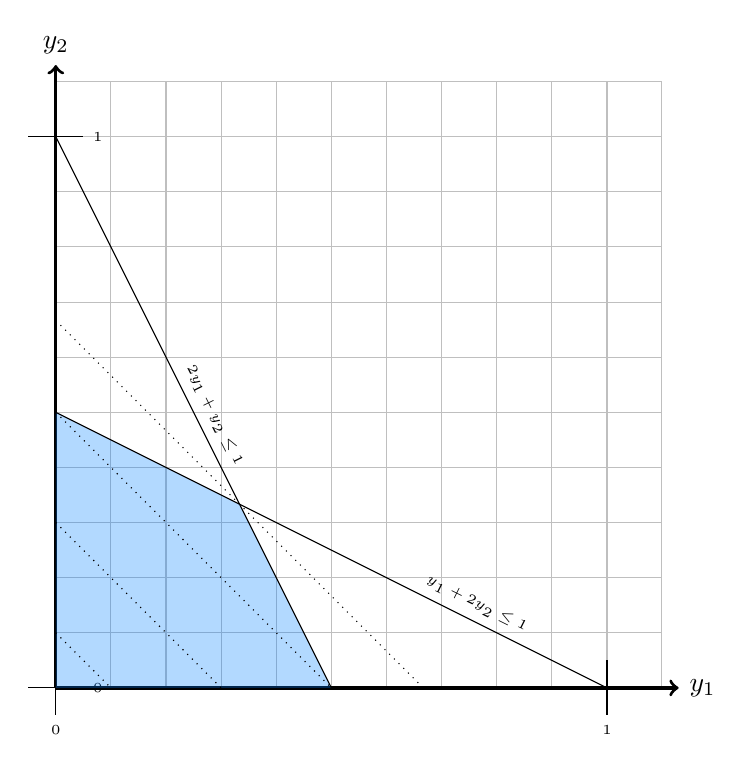
\begin{tikzpicture}[scale=7]

			    \draw[gray!50, thin, step=0.1] (0,0) grid (1.1,1.1);
			    \draw[very thick,->] (0,0) -- (1.13,0) node[right] {$y_1$};
			    \draw[very thick,->] (0,0) -- (0,1.13) node[above] {$y_2$};

			    \foreach \x in {0,...,1.5} \draw (\x,0.05) -- (\x,-0.05) node[below] {\tiny\x};
			    \foreach \y in {0,...,1.5} \draw (-0.05,\y) -- (0.05,\y) node[right] {\tiny\y};

			    \fill[blue!50!cyan,opacity=0.3] (0,0) -- (0,.5) -- (1/3,1/3) -- (.5, 0) -- cycle;

			    \draw (0, .5) -- (.5, .25) -- node[above,sloped] {\tiny$y_1+2y_2\leq1$} (1,0);
			    \draw (0, 1) -- (.125, .75) -- node[above left,sloped] {\tiny$2y_1+y_2\leq1$} (.5, 0);
			    
			    \draw[dotted] (0, .1) -- (.1, 0);
			    \draw[dotted] (0, .3) -- (.3, 0);
			    \draw[dotted] (0, .5) -- (.5, 0);
			    \draw[dotted] (0, 2/3) -- (2/3, 0);

			\end{tikzpicture}

			We can see from the dotted lines I've drawn in for different values of $c$ in\\ $3y_1 + 3y_2 = c$ 
			that the maximum $c$ we will have is the top dotted line when\\ $c = 2, y_1 = 1/3, y_2 = 1/3$.

		\item{(c)} Use the solution you obtained in (b) to get a solution for the primal problem.

			Since both $y_1$ and $y_2$ are non-zero, both inequalities in the primal will be tight. So we get the set of linear equations:

			\begin{align*}
			& x_1+2x_2 = 3\\
			&2x_1+x_2 = 3\\
			\end{align*}

			Which will give us $(x_1, x_2) = (1, 1)$ and an optimal value of 2.
	\end{description}

\end{problem}


\small
\bibliographystyle{amsalpha}
\bibliography{ref}


\end{document}





